\chapter{Arhitektura i dizajn sustava}

    \begin{figure}[!h]
		\centering
		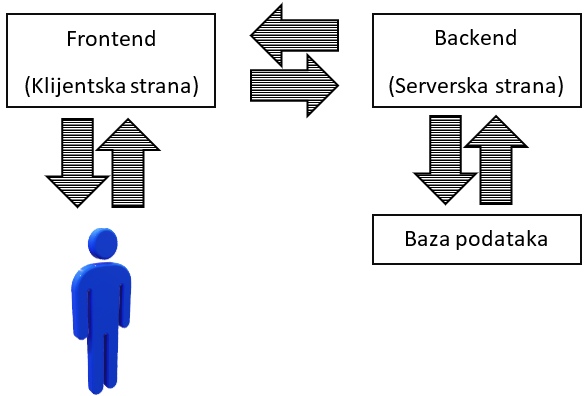
\includegraphics[width=13cm]{slike/arhitektura.PNG} 
		\caption{Arhitektura sustava}
		\label{fig:arhitektura}
	\end{figure}

	Korisnik aplikaciji pristupa putem web preglednika. Interakciju s aplikacijom ostvaruje preko korisničkog sučelja pomoću kojeg šalje zahtjeve web poslužitelju i prima odgovore.\\
Programski jezik pomoću kojeg je ostvaren backend web aplikacije je Java, a korišteni radni okvir je Spring Boot. Frontend aplikacije ostvaren je programskim jezikom JavaScript i bibliotekom React.js. Za razvojno okruženje odabran je Intellij IDEA. Spring Boot je radni okvir namijenjen stvaranju mikroservisa. Mikroservis je arhitektura koja omogućuje neovisan razvoj više različitih servisa od kojih svaki ima svoj proces.\\
Web aplikaciju čine tri osnovna dijela:
	\begin{itemize}
		\item 	\textbf{frontend}
		\item 	\textbf{backend}
		\item 	\textbf{baza podataka }		
	\end{itemize}
Frontend se sastoji od komponenata i logike. Istu komponentu je moguće koristiti za različite namjene (engl. reusability). React.js koristi virtualni DOM (engl. Document Object Model) čiji se sadržaj uspoređuje sa stvarnim DOM-om i na osnovu toga se provode promjene što za posljedicu ima poboljšanje performansi. Struktura ostvarena međusobnim povezivanjem različitih komponenti je stablo.\\
Backend se sastoji od: 
\begin{itemize}
		\item 	programskog sučelja za reprezentacijski prijenos stanja (REST API), odnosno Controller-a
		\item 	sloja poslovne logike (Service)
		\item 	sloja za pristup bazi podataka (Repository)		
	\end{itemize}
\textbf{Controller} izlaže funkcionalnost web aplikacije kao RESTful web usluge, tj. prima zahtjeve čiji su glavni dijelovi URI, metoda i HTTP zaglavlje, a korisniku šalje odgovor koji se sastoji od statusnog koda, tijela poruke i zaglavlja. U tijelu poruke se nalazi sadržaj kojeg korisnik konzumira nakon što je prikazan u web pregledniku. Komunikaciju sa slojem poslovne logike Controller ostvaruje pomoću umetanja ovisnosti (engl. dependency injection). Dependency injection je obrazac prema kojemu se u određeni objekt/funkciju umeće neki drugi objekt/funkcija na koji se prvobitno spomenuti objekt/funkcija oslanja.\\
\textbf{Service} omogućuje komunikaciju između slojeva Controller i Repository, zadužen je za provjeru ispravnosti podataka. Osim na sloju Service, provjera ispravnosti se obavlja na frontend-u i u bazi podataka. Komunikaciju sa slojem za pristup bazi podataka ostvaruje umetanjem ovisnosti.\\ 
\textbf{Repository} omogućuje komunikaciju s bazom podataka pomoću SQL-a. Objekti iz relacijske baze podataka pretvaraju se objekte programskog jezika Java korištenjem tehnike ORM.\\\\
		


		
		\textbf{\textit{dio 1. revizije}}\\

		\textit{ Potrebno je opisati stil arhitekture te identificirati: podsustave, preslikavanje na radnu platformu, spremišta podataka, mrežne protokole, globalni upravljački tok i sklopovsko-programske zahtjeve. Po točkama razraditi i popratiti odgovarajućim skicama:}
	\begin{itemize}
		\item 	\textit{izbor arhitekture temeljem principa oblikovanja pokazanih na predavanjima (objasniti zašto ste baš odabrali takvu arhitekturu)}
		\item 	\textit{organizaciju sustava s najviše razine apstrakcije (npr. klijent-poslužitelj, baza podataka, datotečni sustav, grafičko sučelje)}
		\item 	\textit{organizaciju aplikacije (npr. slojevi frontend i backend, MVC arhitektura) }		
	\end{itemize}

	
		

		

				
		\section{Baza podataka}
			
			\textbf{\textit{dio 1. revizije}}\\
			
		\textit{Potrebno je opisati koju vrstu i implementaciju baze podataka ste odabrali, glavne komponente od kojih se sastoji i slično.}

		Baza podataka za aplikaciju implementirana je u obliku relacijske baze podataka, koja podatke sprema u obliku redaka ili n-torki i stupaca ili atributa koji zajedno tvore tablicu.  \\
Glavna komponenta baze je tablica Korisnik, koja se puni osobnim podacima unesenim pri registraciji u sustav.  Svakom novom korisniku dodjeljuje se primarni ključ, unikatan identifikacijski broj pomoću kojeg se korisnici u bazi podataka međusobno razlikuju. Budući da korisnik ima jednu ili više dodijeljenih uloga, koje su definirane u tablici Uloga, izrađena je veza između dvije tablice koja sadrži identifikacijske brojeve korisnika i odgovarajuće uloge. \\
Kako bi korisnik zaigrao na kvizu, potrebno je prvo pronaći ekipu kojoj odgovara svojim područjima znanja, zbog čega je izrađena tablica Ekipa koja sadrži minimalno jednoga, a maksimalno petero članova.  \\
Ako korisnik ima ulogu sastavljača, on kreira kviz s podacima i informacijama koji se spremaju u tablicu Kviz.  Svaki kviz ima svoj identifikacijski broj i unikatne atribute, vrijeme održavanja i ID sastavljača, jer jedan sastavljač ne može objaviti dva različita kviza koja se održavaju u isto vrijeme.  \\
Tablica Obavijest sadrži svoj identifikacijski broj, tekst obavijesti koji se prikazuje korisniku i ID korisnika kao strani ključ. \\

		
			\subsection{Opis tablica}
			

				\textit{Svaku tablicu je potrebno opisati po zadanom predlošku. Lijevo se nalazi točno ime varijable u bazi podataka, u sredini se nalazi tip podataka, a desno se nalazi opis varijable. Svjetlozelenom bojom označite primarni ključ. Svjetlo plavom označite strani ključ}
				
			
				\begin{longtblr} [
					label = none,
					entry = none
					] {
						width = \textwidth,
						colspec = {|X[8,l]|X[8, l]|X[16, l]|},
						rowhead = 1,
					}
					\hline \textbf{Korisnik} & \\ \hline[3pt]
					\SetCell{LightGreen}korisnik\_id & BIG INT & Identifikacijski broj korisnika, primarni ključ.\\ \hline
					ime & VARCHAR(100) & Ime korisnika. \\ \hline
					prezime & VARCHAR(100) & Prezime korisnika. \\ \hline
					email\_adresa & VARCHAR(100) & E-mail adresa korisnika. \\ \hline
					lozinka & VARCHAR(50) & Lozinka koju korisnik osmisli pri registraciji. \\ \hline
					slika & VARBINARY & Profilna slika korisnika u aplikaciji, opcionalno. \\ \hline
					broj\_telefona & VARCHAR(50) & Broj telefona korisnika, opcionalno. \\ \hline
					podrucja\_znanja & VARCHAR(150) & Područja znanja igrača, koriste se pri odabiru ekipe. \\ \hline
					nadimak(U) & VARCHAR(50) & Nadimak koji si korisnik osmisli pri registraciji. \\ \hline
					prosj\_broj\_ekipa & INT & Prosječan broj ekipa koji sudjeluju u kvizovima nekog sastavljača, opcionalno. \\ \hline
					blokiran & BOOLEAN & Atribut koji daje informaciju o tome je li korisnik blokiran ili ne. \\ \hline
					\SetCell{LightBlue}ekipa\_id & BIG INT & Identifikacijski broj ekipe kojoj korisnik pripada, opcionalno. \\ \hline
				\end{longtblr}

				\begin{longtblr}[
					label = none,
					entry = none
				]{
					width = \textwidth,
					colspec = {|X[8,l]|X[8, l]|X[16, l]|},
					rowhead = 1,
                         		}
				\hline \textbf{Uloga} & \\ \hline[3pt]
				\SetCell{LightGreen} uloga\_id & BIG INT & Identifikacijski broj uloge. \\ \hline
				uloga\_ime & VARCHAR(50) & Ime uloge. \\ \hline
				\end{longtblr}



			
				\begin{longtblr}[
					label = none, 
					entry = none
					]{
						width = \textwidth,
						colspec = {|X[8,l]|X[8, l]|X[16, l]|},
						rowhead = 1,
					}
					\hline \textbf{korisnik\_uloga} & \\ \hline[3pt]
					\SetCell{LightBlue} uloga\_id & BIG INT & Identifikacijski broj uloge, strani ključ s referencom na ulogu.\\ \hline
					\SetCell{LightBlue} korisnik\_id & BIG INT & Identifikacijski broj korisnika, strani ključ s referencom na korisnika. \\ \hline
				\end{longtblr}
			
				\begin{longtblr} [
					label = none, 
					entry = none
					]{
						width = \textwidth,
						colspec = {|X[8,l]|X[8, l]|X[16, l]|},
						rowhead = 1,
					}
					\hline \textbf{Ekipa} & \\ \hline[3pt]
					\SetCell{LightGreen} ekipa\_id & BIG INT & Identifikacijski broj ekipe, primarni ključ. \\ \hline
					broj\_clanova & INT & Broj članova ekipe, ne smije biti manji od 1 ni veći od 5. \\ \hline
					naziv\_ekipe & VARCHAR(50) & Ime ekipe. \\ \hline
				\end{longtblr}
			
			\begin{longtblr} [
				label = none,
				entry = none
				]{
					width = \textwidth,
					colspec = {|X[8,l]|X[8, l]|X[16, l]|},
					rowhead = 1,
				}
			\hline \textbf{Kviz} & \\ \hline[3pt]
			\SetCell{LightGreen} kviz\_id & BIG INT & Identifikacijski broj kviza, primarni ključ. \\ \hline
			kratki\_opis & VARCHAR(200) & Sažeti tekst o sadržaju kviza. \\ \hline
			ime\_kafica & VARCHAR(50) & Ime kafića u kojem se kviz održava. \\ \hline
			vrijeme\_odrzavanja (U) & TIMESTAMP & Vrijeme održavanja kviza, unikatan atribut zajedno s identifikacijskim brojem sastavljača. \\ \hline
			lokacija & GEOGRAPHY & Lokacija mjesta održavanja. \\ \hline
			maks\_broj\_ekipa & INT & Maksimalni broj ekipa koje sudjeluju na kvizu. \\ \hline
			kotizacija & FLOAT & Kotizacija za sudjelovanje na kvizu. \\ \hline
			nagrade & VARCHAR(100) & Popis nagrada na visoko plasirane ekipe. \\ \hline
			vrsta & VARCHAR(50) & Vrsta kviza (povijest, sport, ..). \\ \hline
			naziv\_kviza (U) & VARCHAR(50) & Unikatan naziv kviza. \\ \hline
			aktivan & BOOLEAN & Predstavlja je li kviz trenutno aktivan ili ne. \\ \hline
			\SetCell{LightBlue} korisnik\_id & BIG INT & Identifikacijski broj sastavljača, strani ključ s referencom na korisnika. \\ \hline
			\end{longtblr}

			

			\begin{longtblr}[
				label = none,
				entry = none
			]{
				width = \textwidth,
				colspec = {|X[8,l]|X[8, l]|X[16, l]|},
				rowhead = 1,
			}
			\hline \textbf{sudjeluje\_u} & \\ \hline[3pt]
			\SetCell{LightBlue} ekipa\_id & BIG INT & Identifikacijski broj ekipe, strani ključ s referencom na ekipu. \\ \hline
			\SetCell{LightBlue} kviz\_id & BIG INT & Identifikacijski broj kviza na kojem sudjeluje ekipa, strani ključ. \\ \hline
			\end{longtblr}

			\begin{longtblr} [
				label = none,
				entry = none
			]{
				width = \textwidth,
				colspec = {|X[8,l]|X[8, l]|X[16, l]|},
				rowhead = 1,
			}
			\hline \textbf{Obavijest}& \\ \hline[3pt]
			\SetCell{LightGreen} obavijest\_id & BIG INT & Identifikacijski broj obavijesti, primarni ključ. \\ \hline
			tekst & VARCHAR(300) & Tekst obavijesti. \\ \hline
			\SetCell{LightBlue} korisnik\_id & BIG INT & Identifikacijski broj korisnika koji je primio obavijest. \\ \hline
			\end{longtblr}
			
			
				
				
			
			\subsection{Dijagram baze podataka}
				\textit{ U ovom potpoglavlju potrebno je umetnuti dijagram baze podataka. Primarni i strani ključevi moraju biti označeni, a tablice povezane. Bazu podataka je potrebno normalizirati. Podsjetite se kolegija "Baze podataka".}
			 \begin{figure}[!h]
			\centering
			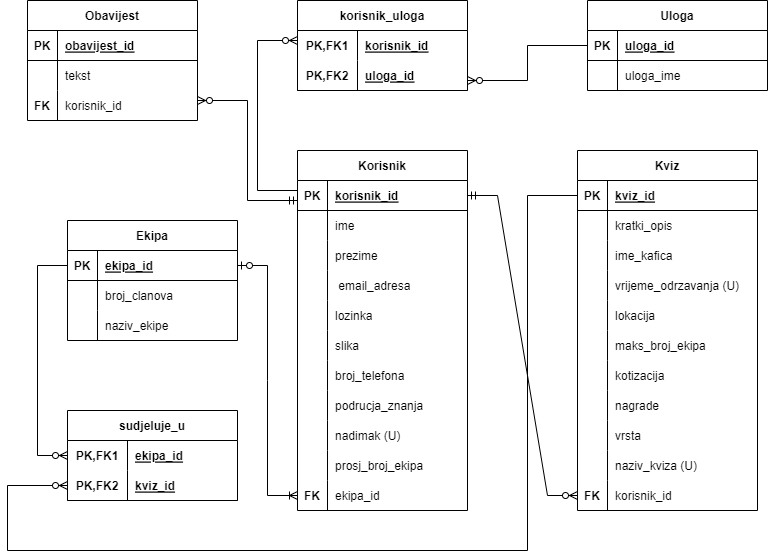
\includegraphics[width=15cm]{slike/final.png} 
			\caption{ER dijagram}
			\label{fig:arhitektura}
	\end{figure}
			
			\eject
			
			
		\section{Dijagram razreda}
		
			\textit{Potrebno je priložiti dijagram razreda s pripadajućim opisom. Zbog preglednosti je moguće dijagram razlomiti na više njih, ali moraju biti grupirani prema sličnim razinama apstrakcije i srodnim funkcionalnostima.}\\
			
			\textbf{\textit{dio 1. revizije}}\\
			
			\textit{Prilikom prve predaje projekta, potrebno je priložiti potpuno razrađen dijagram razreda vezan uz \textbf{generičku funkcionalnost} sustava. Ostale funkcionalnosti trebaju biti idejno razrađene u dijagramu sa sljedećim komponentama: nazivi razreda, nazivi metoda i vrste pristupa metodama (npr. javni, zaštićeni), nazivi atributa razreda, veze i odnosi između razreda.}\\
			
			\textbf{\textit{dio 2. revizije}}\\			
			
			\textit{Prilikom druge predaje projekta dijagram razreda i opisi moraju odgovarati stvarnom stanju implementacije}
			
			
			
			\eject
		
		\section{Dijagram stanja}
			
			
			\textbf{\textit{dio 2. revizije}}\\
			
			\textit{Potrebno je priložiti dijagram stanja i opisati ga. Dovoljan je jedan dijagram stanja koji prikazuje \textbf{značajan dio funkcionalnosti} sustava. Na primjer, stanja korisničkog sučelja i tijek korištenja neke ključne funkcionalnosti jesu značajan dio sustava, a registracija i prijava nisu. }
			
			
			\eject 
		
		\section{Dijagram aktivnosti}
			
			\textbf{\textit{dio 2. revizije}}\\
			
			 \textit{Potrebno je priložiti dijagram aktivnosti s pripadajućim opisom. Dijagram aktivnosti treba prikazivati značajan dio sustava.}
			
			\eject
		\section{Dijagram komponenti}
		
			\textbf{\textit{dio 2. revizije}}\\
		
			 \textit{Potrebno je priložiti dijagram komponenti s pripadajućim opisom. Dijagram komponenti treba prikazivati strukturu cijele aplikacije.}